\chapter{Distributed Programming (Paradigma ad Attori - Akka)}
\section{Struttura generale dell'applicazione} \label{akka}
Tramite il framework Akka, è possibile realizzare un modello ad attori location-transparent per formare reti p2p (o \textit{cluster}).\newline
\noindent Nella soluzione adottata, ogni nodo del cluster (e quindi ogni giocatore) corrisponde anche ad un attore; tutti gli attori nel sistema hanno lo stesso ruolo e prendono decisioni dettate sia dalle azioni dell'utente sia dallo stato del cluster.
\subsection{Comportamento di un nodo}
\begin{figure}[H]
	\begin{center}
		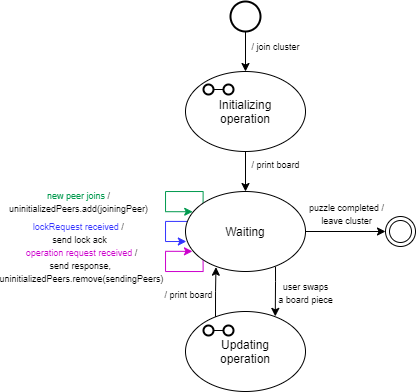
\includegraphics[width=0.6\linewidth]{img/part-2/akka.png}
	\end{center}
	\caption{Diagramma degli stati del comportamento di un nodo nel sistema}
\end{figure}
Un nodo comincia il suo ciclo di vita connettendosi al cluster ed eseguendo un'operazione di inizializzazione del puzzle (\textit{Initializing operation}).\newline
Una volta configurato il puzzle, il nodo entra in stato di attesa, dove permane finché l'utente non decide di muovere un pezzo, iniziando un'operazione di update (\textit{Updating operation}).\newline
Durante il gioco, è possibile ovviamente ricevere richieste riguardo la configurazione corrente (da parte di altri peer che vogliano inizializzarsi) o update su modifiche eseguire dagli altri giocatori.\newline
Nel caso si sia raggiunta la configurazione finale del puzzle il gioco termina, chiudendo l'istanza del programma.\newline

\noindent Trattandosi di un sistema distribuito i cambiamenti alla configurazione corrente del puzzle possono essere eseguiti da uno qualsiasi dei nodi e, conseguentemente, il nuovo stato deve essere propagato a tutti i componenti del cluster, che devono risultare tra loro sincronizzati e consistenti.\newline
\noindent Sorge quindi la necessità di utilizzare meccanismi per la gestione di una sezione critica all'interno della quale un nodo possa eseguire un'operazione atomicamente senza il rischio di interleaving con gli altri nodi del cluster.\newline

\noindent Initializing operation e updating operation dunque utilizzeranno un meccanismo comune per la gestione della sezione critica; il comportamento dettagliato di una operation verrà discusso nella sezione \textit{3.1.3}, ma prima verrà analizzato l'algoritmo distribuito utilizzato.

\subsection{Sezione critica}\label{sezioneCriticaAkka}
Analogamente a quanto visto nella programmazione multi-threaded, una sezione critica garantisce:
\begin{itemize}
    \item \textit{safety} \newline
    Due processi non possono essere in sezione critica contemporaneamente.
    \item \textit{liveness} \newline
    Tutte le richieste di entrare in sezione critica verranno soddisfatte prima o poi.
    \item \textit{fairness} \newline
    Le richieste devono essere soddisfatte nell'ordine di arrivo.
\end{itemize}
Trovandoci in un contesto distribuito, al fine di istituire una sezione critica saranno necessarie tecniche algoritmiche. La parte più difficile in tutto questo però è garantire la fairness, in quanto non vi è un clock condiviso.
\subsubsection{Lamport clock}
Un Lamport clock è una semplice implementazione di clock logico; tramite esso è possibile stabilire un ordine parziale tra gli eventi tramite la relazione happened before.\newline

\noindent Seppur non venga garantito un ordine totale (come ad esempio sarebbe possibile tramite un Vector clock), tale struttura risulta comunque sufficiente in contesti dove la rigidità dell'ordinamento può essere meno stringente.

\subsubsection{Algoritmo di Ricart Agrawala}
Vi sono due categorie di algoritmi, in un contesto distribuito, per la gestione della sezione critica:
\begin{itemize}
    \item \textit{centralizzati} \newline
    Un coordinatore distribuisce il token di accesso alla sezione critica occupandosi di accodare le richieste, garantendone solo una per volta.
    \item \textit{decentralizzati} \newline
    Non è presente nessun coordinatore e un nodo che voglia accedere alla sezione critica dovrà prima ottenere il consenso da parte di tutti gli altri nodi presenti nella rete.
\end{itemize}
L'algoritmo di Ricart Agrawala, utilizzato in questo elaborato, ricade nella seconda categoria.\newline

\noindent Un nodo che voglia richiedere l'accesso alla sezione critica salverà il valore del Lamport clock al momento della richiesta ed invierà a tutti gli altri nodi della rete una richiesta di lock (con allegato il clock della richiesta); il nodo dunque si metterà in attesa degli ack da parte di tutti gli altri nodi.\newline

\noindent Quando un nodo riceve una richiesta di lock invierà un ack nel caso in cui esso non sia interessato ad accedere alla sezione critica oppure nel caso in cui il clock allegato alla richiesta preceda il clock della sua richiesta; se il clock della propria richiesta dovesse invece precedere il clock della richiesta ricevuta, quest'ultima verrà messa in una coda.\newline

\noindent Una volta ricevuti tutti gli ack, un nodo eseguirà la sua operazione in sezione critica e, alla fine, rilascerà il lock inviando un ack a tutte le richieste eventualmente messe in coda.

\subsection{Operazione in CS}
Riconnettendoci a quanto detto nella \textit{sezione 3.1.1}, analizziamo comportamento di una operation (initialize / update).\newline
\noindent Il diagramma mostra un'estensione dell'algoritmo di Agrawala, dove vengono presi in considerazione anche i fallimenti dei nodi (vedi \textit{sezione 3.3.1}), l'ingresso di nuovi nodi nel cluster e il broadcast dei messaggi riguardanti le operazioni concrete una volta ottenuta la sezione critica.\newline

\noindent All'interno del cluster vi saranno due tipologie di nodi:
\begin{itemize}
    \item \textit{initialized}\newline
    Tutti i nodi che hanno già ricevuto la configurazione iniziale.
    \item \textit{uninitialized}\newline
    Tutti i nodi che, viceversa, non hanno ancora ricevuto la configurazione iniziale.
\end{itemize}
Quando un nodo entra all'interno del cluster inizia come nodo uninitialized. Una volta che tale nodo abbia completato con successo un'operazione (necessariamente la sua prima operazione sarà l'inizializzazione) verrà promosso ad initialized.\newline
Tale distinzione risulta fondamentale, ad esempio, nel caso tutti i nodi rimasti all'interno del cluster siano uninitialized; il nodo con l'operazione di inizializzazione più vecchia, rendendosi conto che non esiste possibilità di reperire una configurazione del puzzle, ne creerà una nuova casuale.\newline

\begin{figure}[H]
	\begin{center}
		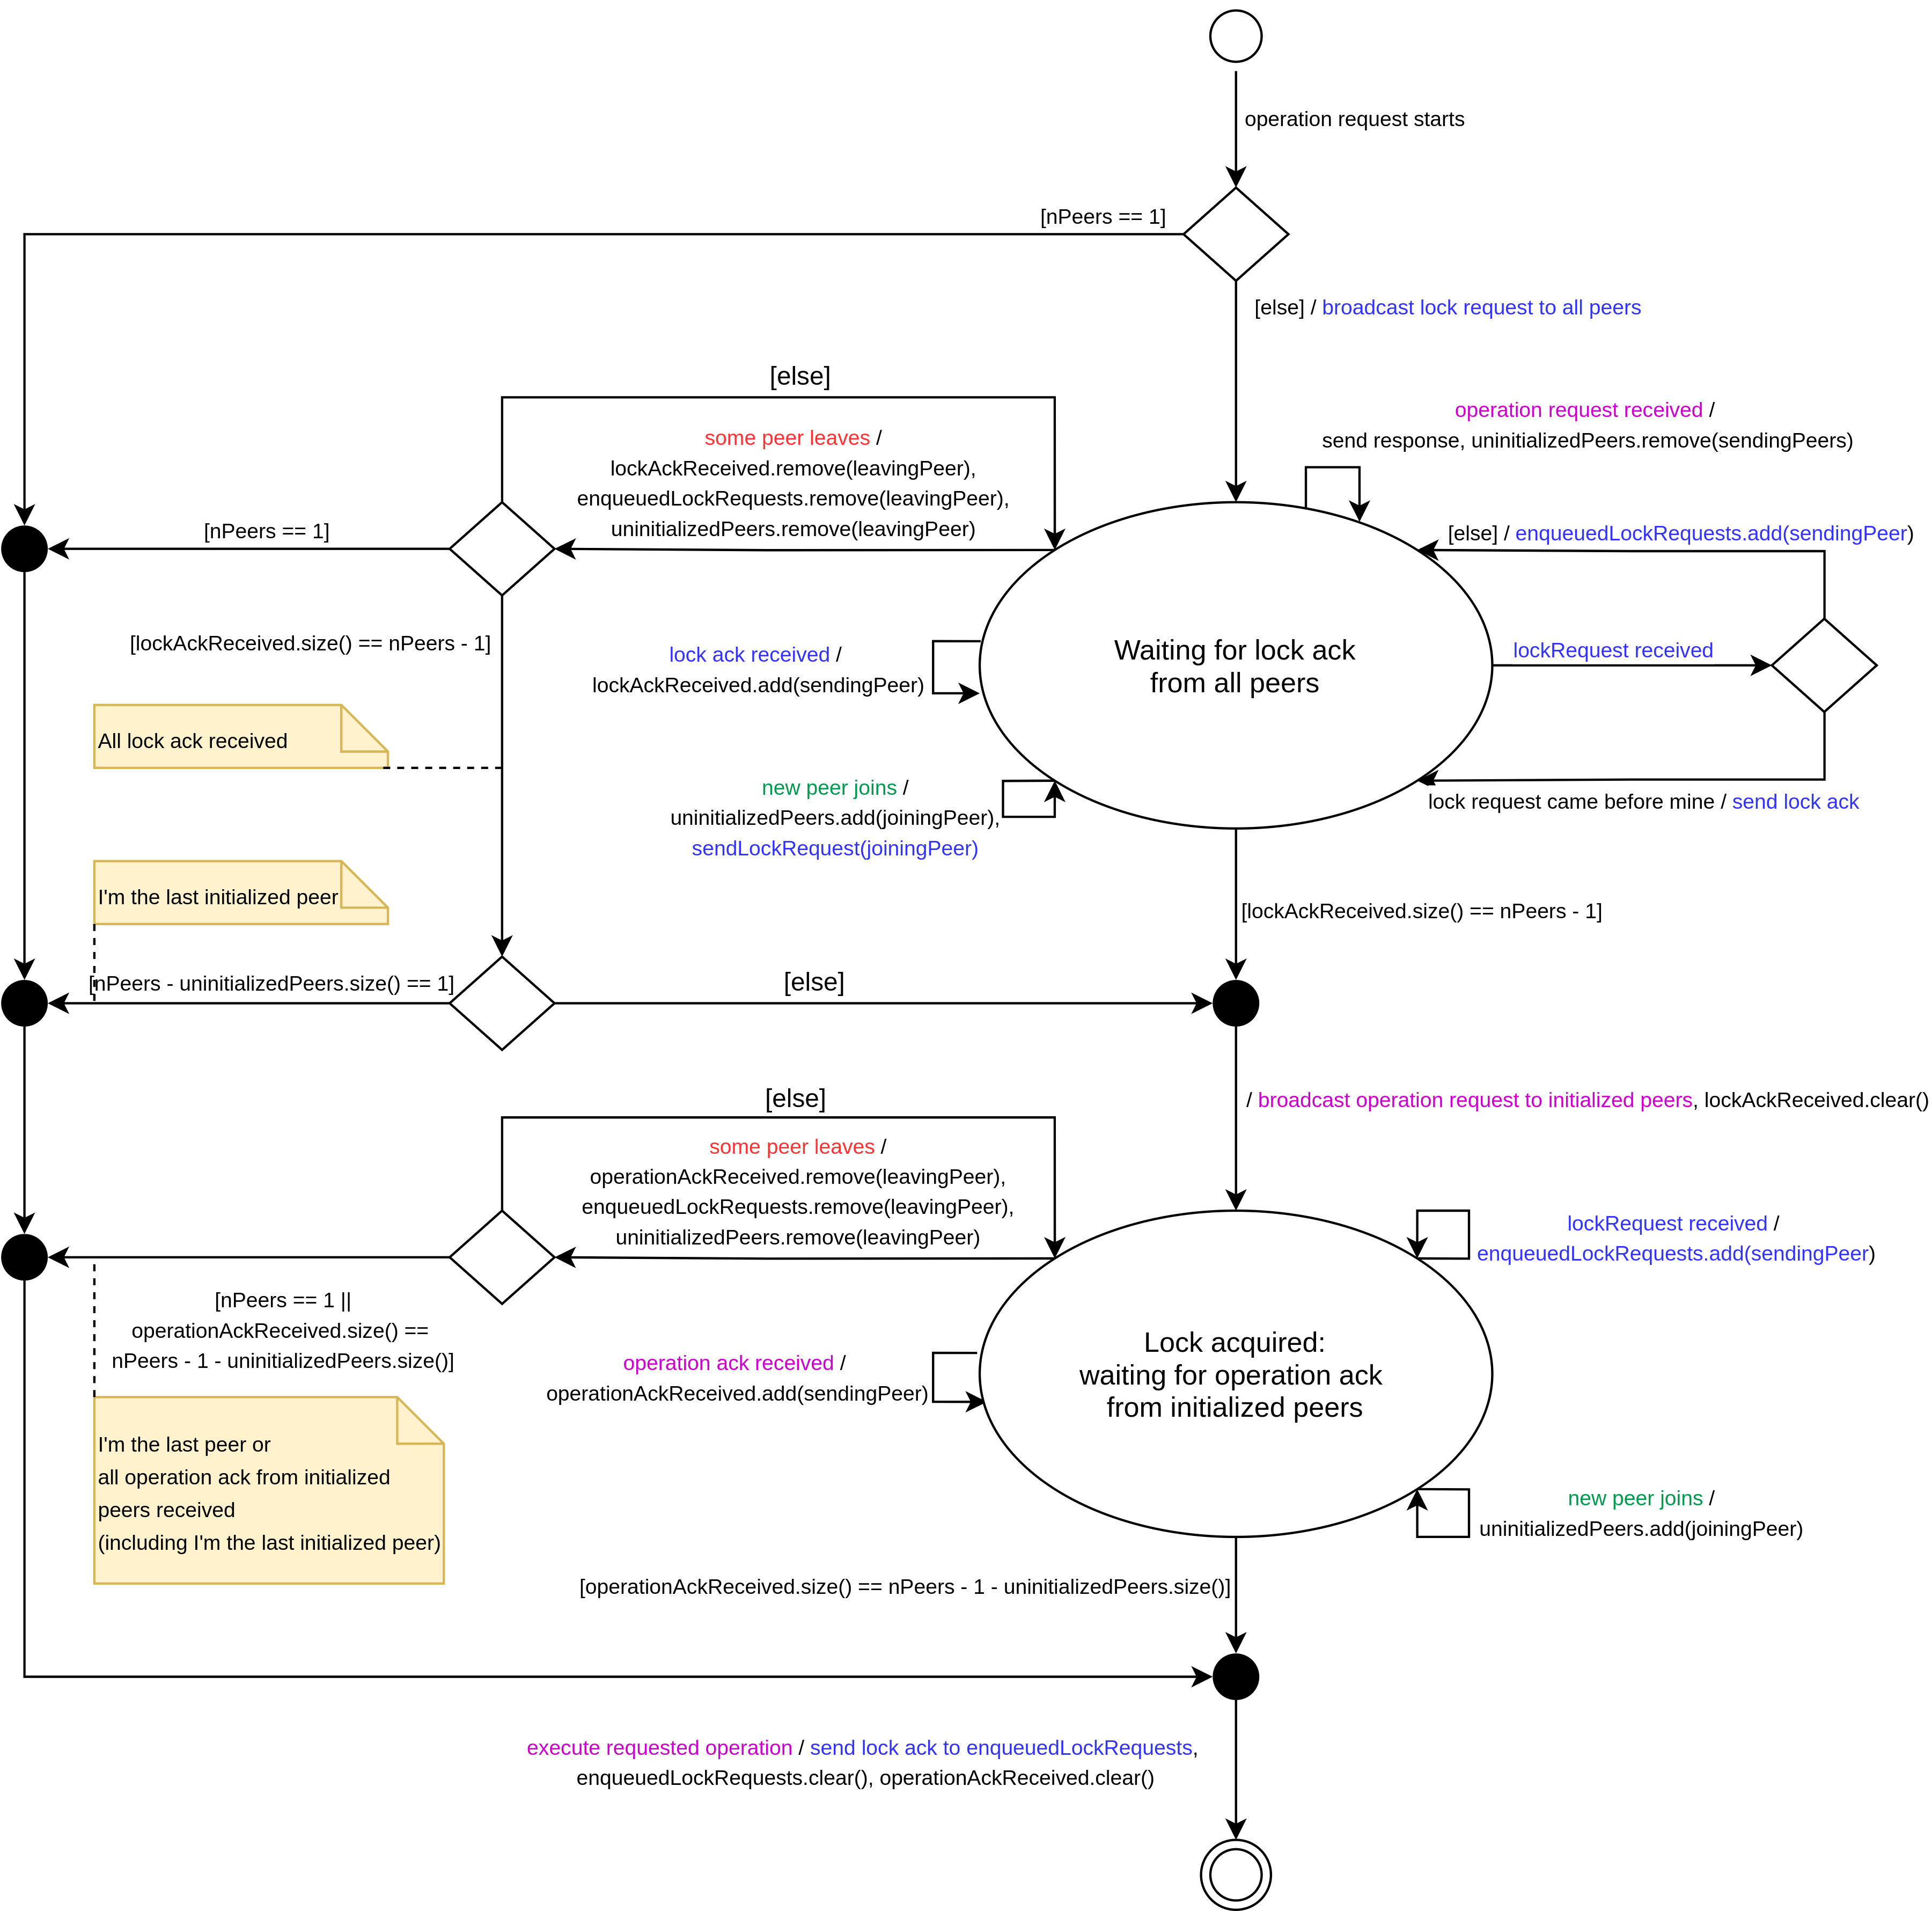
\includegraphics[width=1\linewidth]{img/part-2/operation.png}
	\end{center}
	\caption{Diagramma degli stati dettagliato del comportamento di un nodo nel sistema}
\end{figure}

\noindent Una operation dunque si svolge in due step:
\begin{itemize}
    \item \textit{Waiting for lock ack from alla peers} \newline
    In questo stato è stata iniziata la richiesta della sezione critica e si attende dunque l'ack da tutti i peer.\newline
    Nel caso un nuovo nodo entri nel cluster in questa fase sarà necessario inviare anche ad esso una richiesta di lock.\newline
    Nel caso si riceva una richiesta di operazione (inviare la situazione corrente del puzzle oppure aggiornare tale situazione), essa dovrà essere soddisfatta rimandando indietro una conferma adeguata al tipo di operazione.\newline
    L'uscita/fallimento di un nodo sarà trattata nella \textit{sezione 3.3.1}.
    \item \textit{Lock acquired: waiting for operation ack from initialized peers}\newline
    Una volta ottenuta la sezione critica, l'operazione sarà propagata a tutti i nodi initialized.\newline
    Inviare il messaggio anche ai nodi uninitialized risulterebbe inutile, in quanto in un'operazione di update un nodo uninitialized non disporrebbe di una configurazione sulla quale applicare i cambiamenti; nel caso di un'operazione di inizializzazione, invece, risulterebbe inutile chiedere la configurazione corrente del puzzle a dei nodi che non la posseggono.\newline
    Una volta ricevuto l'ok da tutti i nodi initialized, lo stato globale sarà sincronizzato e il nodo potrà rilasciare il lock della sezione critica, inviando il suo ack a tutti i nodi che nel mentre abbiano fatto richiesta di accedervi.
\end{itemize}
Nel caso in cui il nodo sia l'unico della rete tali fasi saranno ovviamente saltate (in quanto non sarà necessario richiedere l'accesso alla sezione critica) e l'operazione verrà eseguita immediatamente.

\section{Messaggi}
All'interno del sistema viaggiano messaggi appartenenti a una delle seguenti categorie:
\begin{itemize}
    \item \textit{Akka cluster events}\newline
    Messaggi integrati nel framework Akka i quali notificano riguardo cambiamenti nella configurazione del cluster.
    \item \textit{Puzzle messages}\newline
    Messaggi da noi ideati per rispondere alle necessità dell'applicativo. Ogni Puzzle message allega un Lamport clock.
\end{itemize}
\subsection{Akka cluster events}
\begin{itemize}
    \item \textbf{MemberUp}\newline
    Scatenato quando un nuovo nodo entra a far parte del cluster.
    \item \textbf{UnreachableMember}\newline
    Scatenato nel caso un nodo non sia più raggiungibile.
    \item \textbf{MemberRemoved}\newline
    Scatenato nel momento in cui un nodo esca dal cluster.
\end{itemize}
\subsection{Puzzle messages}
\begin{itemize}
    \item \textbf{AskLock}\newline
    Inviato a tutti i nodi del cluster da parte di chi voglia accedere alla sezione critica.
    \item \textbf{GrantLock}\newline
    Inviato come risposta ad un AskLock nel momento in cui un nodo sia disponibile a fornire il proprio consenso all'accesso alla sezione critica.
    \item \textbf{InitializeBoardRequest}\newline
    Inviato in broadcast a tutti i nodi initialized da un nodo che abbia ottenuto la sezione critica e voglia ottenere la configurazione corrente del puzzle.
    \item \textbf{InitializeBoardAck}\newline
    Inviato come risposta a un InitializeBoardRequest, allegando la configurazione corrente.
    \item \textbf{UpdateBoardRequest}\newline
    Inviato in broadcast a tutti i nodi initialized da un nodo che abbia ottenuto la sezione critica e che voglia modificare la configurazione corrente del puzzle.
    \item \textbf{UpdateBoardAck}\newline
    Inviato come risposta ad una UpdateBoardRequest.
\end{itemize}
\section{Gestione dei fallimenti} \label{fallimentiAkka}
\subsection{Crash di un nodo}
Nel momento in cui un'istanza di un client venga chiusa volontariamente da un utente, un messaggio di MemberRemoved verrà propagato automaticamente da Akka verso tutti i nodi ancora presenti nel cluster; nel caso un client però incomba in un crash o perda la connessione, allora esso andrà in uno stato unreachable, scatenando in Akka un messaggio UnreachableMember. La politica da noi adottata in questo caso è che, nel caso un nodo sia unreachable, esso verrà escluso dal cluster, arrivando nuovamente a scatenare una MemberRemoved.\newline

\noindent Tornando al diagramma nella \textit{sezione 3.1.3}, ciò che succederà nel caso un nodo esca dal cluster varierà leggermente dipendentemente dallo stato.\newline
Due operazioni verranno sempre eseguite:
\begin{itemize}
    \item rimozione di un'eventuale richiesta di sezione critica (associata a quel nodo) in coda
    \item rimozione del nodo dalla lista dei nodi non inizializzati
\end{itemize}
Nel caso la sezione critica non sia ancora stata ottenuta, un eventuale ack ricevuto dal nodo uscente verrà rimosso dalla lista; analogamente, nel caso la sezione critica sia già stata ottenuta e si stia eseguendo un operazione, l'eventuale ack verrà eliminato. Entrambe le operazioni vengono eseguite al fine di decidere se non sia più necessario attendere ulteriori ack.
\subsection{Akka seeds}
Nel framework Akka, non tutti i nodi hanno la stessa importanza nella creazione di un cluster.\newline
Vi sono alcuni nodi particolari denominati \textbf{seed}; tali nodi costituiscono gli snodi centrali sulla quale il cluster è formato. Essi devono avere un ID e un indirizzo noto.\newline

\noindent I nodi seed cercano costantemente di connettersi tra loro, creando il cluster (è sufficiente un solo seed per avere un cluster); analogamente un nodo NON seed cercherà di accedere al cluster contattando uno qualsiasi tra i cluster.\newline

\noindent Una rete cluster in questo caso però è resistente proporzionalmente al numero dei suoi seed. Un seed che non sia raggiungibile inoltre non è utilizzabile per la gestione del cluster. Una rete cluster in Akka dunque possiede al massimo N nodi seed, con N a calare dipendentemente dal numero di peer attivi/raggiungibili.\newline

\noindent Quanto detto porta a due meccanismi importanti da tenere in considerazione:
\begin{itemize}
    \item Ne nessun seed è raggiungibile, non sarà possibile formare un cluster.
    \item Nel caso un cluster sia già formato, se nessun nodo seed rimane all'interno della rete essa diviene irraggiungibile (le connessioni tra i nodi presenti continueranno a funzionare, ma nessun nodo si potrà più aggiungere a quel cluster). Nel caso un seed torni disponibile successivamente, esso formerà comunque un nuovo cluster in quanto i seed precedenti non sono più raggiungibili.
\end{itemize}
